\subsubsection{UC\theuccount-PG - GitLab invia segnalazione al Producer GitLab}
%	\begin{figure}[H]
%		\centering
%		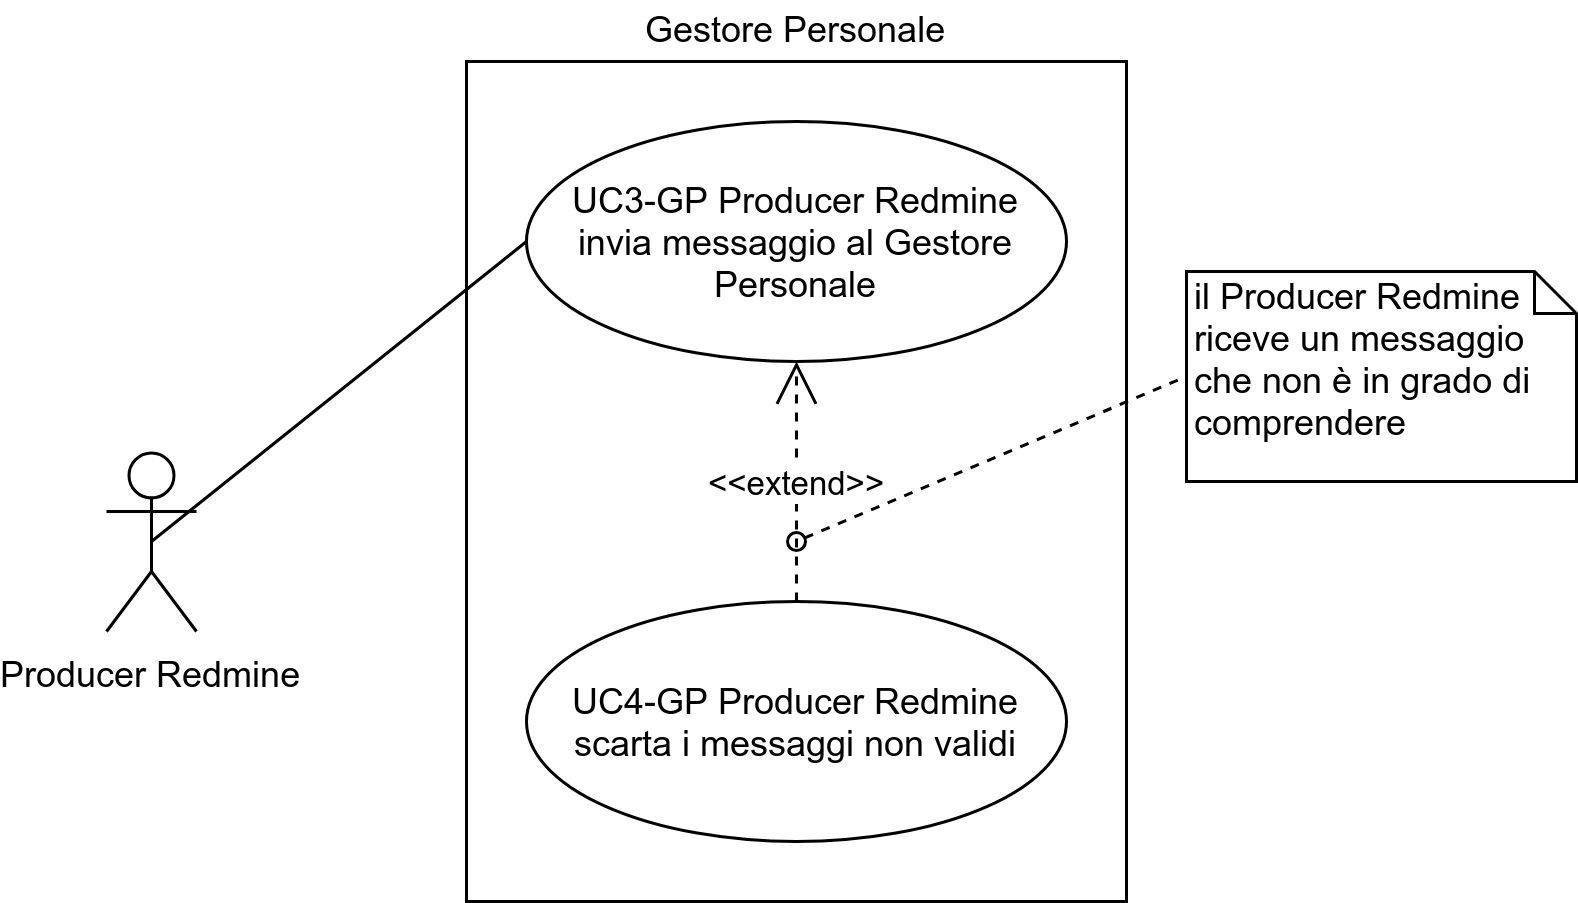
\includegraphics[width=0.5\textwidth]{img/casi_d'uso/UC4.png}\\
%		\caption{UC\theuccount-PG - GitLab segnala apertura issue al Producer GitLab}
%	\end{figure}
\begin{itemize}
    \item \textbf{Codice}: UC\theuccount-PG.
    \item \textbf{Titolo}: GitLab invia segnalazione al Producer GitLab.
    \item \textbf{Attori primari}: GitLab.
    \item \textbf{Descrizione}: GitLab invia una segnalazione tramite webhook a \progetto.
    \item \textbf{Precondizione}: su GitLab viene eseguita una operazione che scaturisce una
    segnalazione da inviare a \progetto.
    \item \textbf{Postcondizione}: il Producer GitLab riceve la segnalazione da GitLab.
    \item \textbf{Scenario principale}: 
    \begin{enumerate}
        \item Viene eseguita un'operazione
        \item GitLab procede all'invio della segnalazione al Producer GitLab
        \item Il Producer GitLab riceve la segnalazione
    \end{enumerate}
    
\end{itemize}

\stepcounter{subuccount}

\subsubsection{UC\theuccount.\thesubuccount-PG - GitLab segnala apertura issue al Producer GitLab}
%	\begin{figure}[H]
%		\centering
%		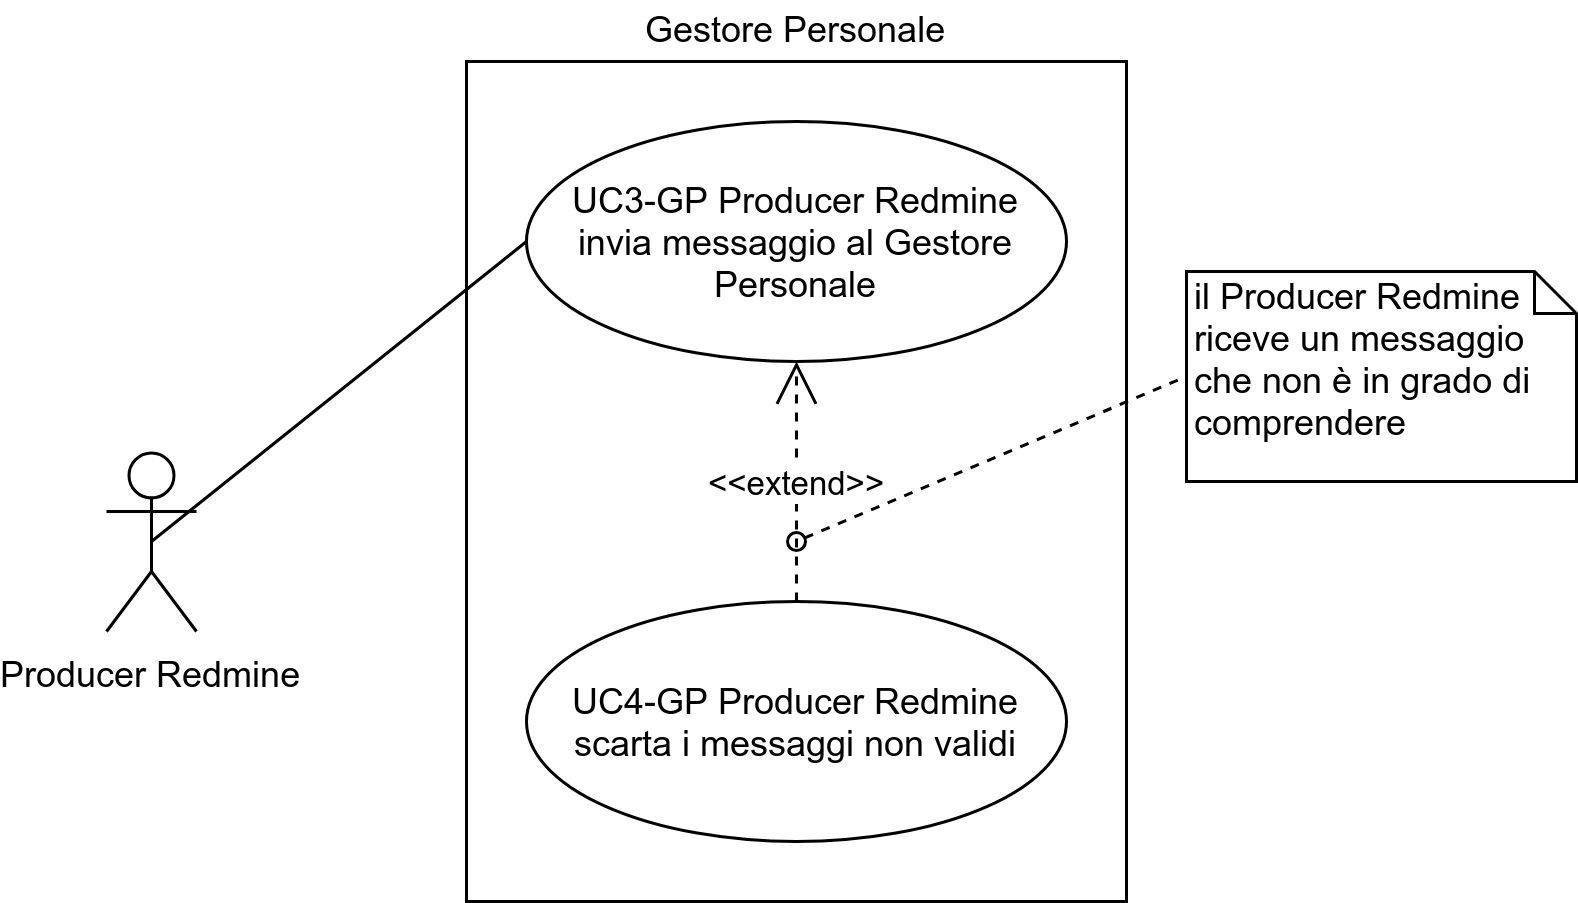
\includegraphics[width=0.5\textwidth]{img/casi_d'uso/UC4.png}\\
%		\caption{UC\theuccount-PG - GitLab segnala apertura issue al Producer GitLab}
%	\end{figure}
\begin{itemize}
    \item \textbf{Codice}: UC\theuccount.\thesubuccount-PG.
    \item \textbf{Titolo}: GitLab segnala apertura issue al Producer GitLab.
    \item \textbf{Attori primari}: GitLab.
    \item \textbf{Descrizione}: GitLab segnala l'apertura di una nuova issue tramite webhook a \progetto.
    L'apertura di una issue su GitLab contiene:
    \begin{itemize}
        \item Object kind
        \item Action
        \item Project
        \item Title e opzionalmente:
        \begin{itemize}
            \item Label
            \item Milestone
            \item Assignees
            \item Due Date
        \end{itemize}
    \end{itemize}
    Il campo object kind ci permette di capire il tipo di oggetto, in questo caso infatti contiene ``issue'', mentre il campo action ha ``open''.
    \item \textbf{Precondizione}: viene aperta una issue su GitLab da 
    segnalare a \progetto.
    \item \textbf{Postcondizione}: il Producer GitLab riceve la segnalazione da GitLab.
    \item \textbf{Scenario principale}: 
    \begin{enumerate}
        \item Viene aperta una nuova issue su GitLab
        \item GitLab procede all'invio della segnalazione di issue al Producer GitLab
        \item il Producer GitLab riceve la segnalazione di apertura issue
    \end{enumerate}
    
\end{itemize}

\stepcounter{subuccount}

\subsubsection{UC\theuccount.\thesubuccount-PG - Gitlab segnala la modifica di una issue al Producer Gitlab}
%	\begin{figure}[H]
%		\centering
%		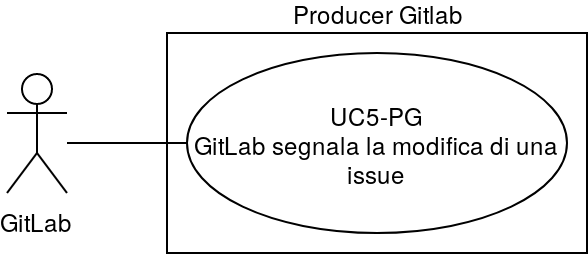
\includegraphics[width=0.5\textwidth]{img/casi_d'uso/UC5.png}\\
%		\caption{UC\theuccount-PG - Gitlab segnala la modifica di una issue al Producer Gitlab}
%	\end{figure}
\begin{itemize}
    \item \textbf{Codice}: UC\theuccount.\thesubuccount-PG.
    \item \textbf{Titolo}: Gitlab segnala la modifica di una issue al Producer Gitlab.
    \item \textbf{Attori primari}: GitLab.
    \item \textbf{Descrizione}: GitLab segnala la modifica di una issue esistente tramite webhook a
    \newline \progetto.
    I campi di interesse sono gli stessi dell'apertura issue, con la differenza che il campo action contiene ``udpate''.
    \item \textbf{Precondizione}: Viene modificata una issue già aperta su un
    progetto di GitLab da segnalare a \progetto.
    \item \textbf{Postcondizione}: il Producer GitLab riceve la segnalazione da GitLab.
    \item \textbf{Scenario principale}: 
    \begin{enumerate}
        \item Viene modificata una issue già esistente su GitLab
        \item GitLab procede all'invio della segnalazione di modifica issue al Producer GitLab
        \item Il Producer GitLab riceve la segnalazione di modifica issue
    \end{enumerate}
    
\end{itemize}

\stepcounter{subuccount}

\subsubsection{UC\theuccount.\thesubuccount-PG - Gitlab segnala il commento di una issue al Producer Gitlab}
%	\begin{figure}[H]
%		\centering
%		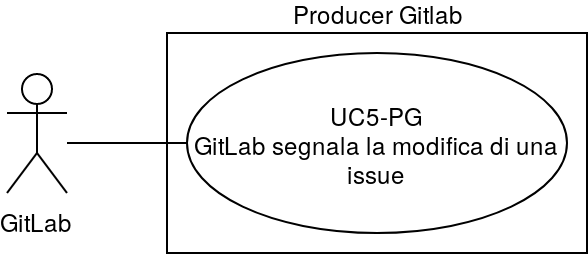
\includegraphics[width=0.5\textwidth]{img/casi_d'uso/UC5.png}\\
%		\caption{UC\theuccount-PG - Gitlab segnala la modifica di una issue al Producer Gitlab}
%	\end{figure}
\begin{itemize}
    \item \textbf{Codice}: UC\theuccount.\thesubuccount-PG.
    \item \textbf{Titolo}: Gitlab segnala il commento di una issue al Producer Gitlab.
    \item \textbf{Attori primari}: GitLab.
    \item \textbf{Descrizione}: GitLab segnala il commento di una issue esistente tramite webhook a \progetto.
    I campi di interesse sono gli stessi dell'apertura issue, con la differenza che il campo action contiene ``issue-note''.
    \item \textbf{Precondizione}: Viene commentata una issue già aperta su un
    progetto di GitLab da segnalare a \progetto.
    \item \textbf{Postcondizione}: il Producer GitLab riceve la segnalazione da GitLab.
    \item \textbf{Scenario principale}: 
    \begin{enumerate}
        \item Viene commentata una issue già esistente su GitLab
        \item GitLab procede all'invio della segnalazione di commento issue al Producer GitLab
    \end{enumerate}
    
\end{itemize}

\stepcounter{subuccount}

\subsubsection{UC\theuccount.\thesubuccount-PG - GitLab segnala un evento di push a Producer GitLab}
%	\begin{figure}[H]
%		\centering
%		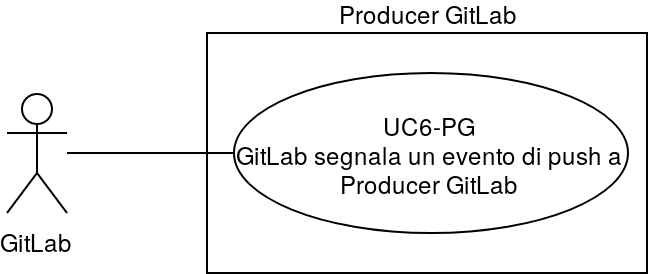
\includegraphics[width=0.5\textwidth]{img/casi_d'uso/UC6.png}\\
%		\caption{UC\theuccount-PG - GitLab segnala un evento di push a Producer GitLab}
%	\end{figure}
\begin{itemize}
\item \textbf{Codice}: UC\theuccount.\thesubuccount-PG.
\item \textbf{Titolo}: GitLab segnala un evento di push a Producer GitLab.
\item \textbf{Attori primari}: GitLab.
\item \textbf{Descrizione}: GitLab segnala un evento di push tramite webhook a \progetto. L'evento di	push può essere composto da uno o più commit.
I campi di interesse sono:
\begin{itemize}
    \item Object kind
    \item Project
    \item Repository
    \item Commits
\end{itemize}
E in questo caso il campo object kind contiene ``push''.
\item \textbf{Precondizione}: Viene effettuato un push su GitLab da segnalare a \progetto.
\item \textbf{Postcondizione}: il Producer GitLab riceve la segnalazione da GitLab.
\item \textbf{Scenario principale}: 
\begin{enumerate}
    \item Viene effettuato un push in GitLab
    \item GitLab procede all'invio della segnalazione di push al Producer GitLab
    \item IlProducer GitLab riceve la segnalazione dell'evento di push
\end{enumerate}

\end{itemize}

\stepcounter{subuccount}

\subsubsection{UC\theuccount.\thesubuccount-PG - Gitlab segnala il commento di un commit al Producer Gitlab}
%	\begin{figure}[H]
%		\centering
%		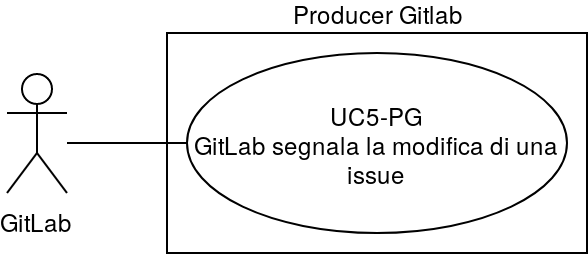
\includegraphics[width=0.5\textwidth]{img/casi_d'uso/UC5.png}\\
%		\caption{UC\theuccount-PG - Gitlab segnala la modifica di una issue al Producer Gitlab}
%	\end{figure}
\begin{itemize}
    \item \textbf{Codice}: UC\theuccount.\thesubuccount-PG.
    \item \textbf{Titolo}: Gitlab segnala il commento di un commit al Producer Gitlab.
    \item \textbf{Attori primari}: GitLab.
    \item \textbf{Descrizione}: GitLab segnala il commento di un commit esistente tramite webhook a \progetto.
    I campi di interesse sono gli stessi dell'apertura issue, con la differenza che il campo action contiene ``commit-note''.
    \item \textbf{Precondizione}: Viene commentato un commit di un progetto di GitLab da segnalare a \progetto.
    \item \textbf{Postcondizione}: il Producer GitLab riceve la segnalazione da GitLab.
    \item \textbf{Scenario principale}: 
    \begin{enumerate}
        \item Viene commentato un commit già esistente su GitLab
        \item GitLab procede all'invio della segnalazione di commento commit al Producer GitLab
        \item Il Producer GitLab riceve la segnalazione di commento di un commit
    \end{enumerate}
    
\end{itemize}
